\section{Die Simulationsumgebung und \enquote{LightJason}}
\label{sec:simulationsumgebung}

Als Simulationsumgebung für die geplanten Tests der Modelle wurde eine modifizierte Version einer Java-Software benutzt, welche im September 2017 für einen Workshop\footnote{siehe \url{https://lightjason.github.io/news/2017-09-workshop/}} mit Doktoranden genutzt wurde.
Die Steuerung des Agentenverhaltens wird dabei von LightJason, vorgestellt in \cite{lightjason}, übernommen.

Es handelt sich um ein BDI-Multi-Agenten-Framework zum Erstellen von Multiagentensystemen mit Java, welches nebenläufige Ausführung unterstützt. 
Dabei wurde versucht einen Rahmen zu schaffen, der es ermöglicht, AI-Algorithmen zu einer bestehenden Softwarearchitektur hinzuzufügen. 
Das Framework kombiniert klassische Methoden der Künstlichen Intelligenz mit Optimierungs- und Fuzzy-Logik-Konzepten.
(nach \cite{lightjason-web})

LightJason beschreibt einen BDI-Agenten als parallel ausgeführten regelbasierten Zustandsautomaten. Somit eignet sich das grundlegende Ausführungskonzept für den Einsatz im Rahmen eines zellulären Automaten (siehe \ref{sec:ca}).



%%%%%%%%%%%%%%%%%%%%%%%%%%%%%%%%%%%%%%%%%%%%%%%%%%%%%%%%%%%
%	NEW SUBSECTION
%%%%%%%%%%%%%%%%%%%%%%%%%%%%%%%%%%%%%%%%%%%%%%%%%%%%%%%%%%%



\subsection[Multiagentensysteme]{Multiagentensysteme (nach \cite{multiagent})}
\label{sec:multiagentensysteme}

Wann immer in der Vergangenheit verteilte Systeme entwickelt wurden, stellte genau diese Verteilung ein Problem dar. 
Wenn ein Computersystem, das in unserem Aufrag handelt, mit einem anderen interagiert, das die Interessen einer anderen Person vertritt, dann ist es ziemlich sicher, dass diese Interessen nicht die gleichen sind.
Es wurde notwendig, die Systeme mit der Fähigkeit auszustatten, mit anderen Systemen zu kooperieren und mit ihnen Übereinkünfte zu erzielen - mehr oder minder in der gleichen Weise wie wir Menschen dies im täglichen Leben tun.

Die Idee eines Multiagentensystems ist dabei recht einfach.
Ein Agent ist ein Computersystem, welches in der Lage ist, selbständig im Interesse seiner Benutzer/Eigner zu handeln.
Der Agent kann eigenständig herausfinden, welche Handlungen nötig sind, um seine Designziele zu erreichen, ohne dass ihm immer wieder vorgegeben werden müsste, was in welchem Moment zu tun ist.

Der Agent ist die aktuell letzte Stufe der Entwicklung in der Reihe der \mbox{Programmierkonzepte -} von Maschinensprache und Assemblercode bis hin zu abstrakten Datentypen und Objekten.

Ein Multiagentensystem besteht in der Regel aus einer Anzahl von Agenten, deren Kommunikation über eine Computernetzwerkinfrastruktur abläuft.
Die Zielsetzung und Motivation der einzelnen Agenten kann grundverschieden sein, da jeder Agent \textls{ sein } Ziel bzw. das seines Benutzers verfolgt.
% Da jeder Agent seine Ziele, bzw. die seines Benutzers, verfolgt, können die Ziele und Motivation der einzelnen Agenten grundverschieden sein. \sa{own: daddy said: Die Ziele und die Motivation der einzelnen Agenten kann grundverschieden sein, da jeder   s e i n  Ziel, bzw. das seines Benutzers verfolgt.}
Für eine Interaktion müssen die Agenten die Fähigkeit haben, zu kooperieren, zu koordinieren und zu verhandeln.

\begin{figure}[hptb]
 \centering
 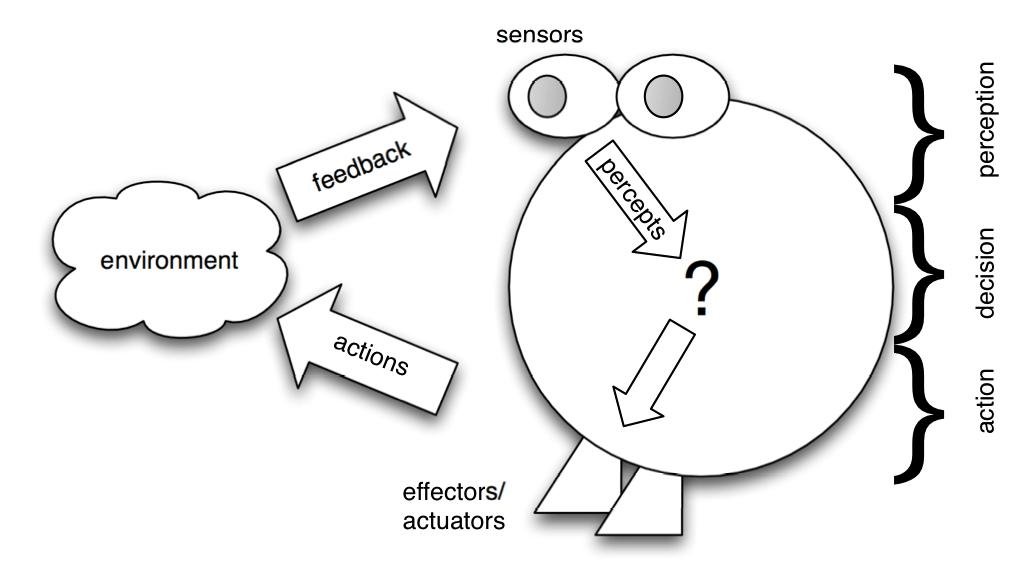
\includegraphics[width=0.9\textwidth]{intelligent-agent}
 \caption[ein Agent in seiner Umwelt]
 		{ein Agent in seiner Umwelt, aus \cite[Figure 2.1]{multiagent}}
 \label{figure:intelligent-agent}
\end{figure}
\noindent
Jeder Agent befindet sich dabei in einer Umwelt, die er mit verschiedenen geigneten Sensoren wahrnehmen kann, siehe \cref{figure:intelligent-agent}.
Dies können bei Agenten in einer realen Umwelt phsysische Sensoren oder bei Softwareagenten Softwaresensoren sein.
\\
Aufgrund dieser Umweltwahrnehmung trifft er Entscheidungen und handelt entsprechend.
% Aufgrund dieser Wahrnehmung seiner Umwelt trifft er Entscheidungen und handelt dann entsprechend dieser. \sa{own: daddy said: Er entscheidet dann aufgrund dieser Umweltwahrnehmung und handelt entsprechend.}
Durch seine Handlungen (und natürlich auch die von anderen Agenten in der gleichen Umwelt) kann diese Umwelt verändert werden.
Dies kann auch während der Entscheidungsfindung des Agenten passieren, so dass die getroffene Entscheidung nicht mehr optimal zum dann aktuellen Zustand der Umwelt ist.

Ein einfaches System, welches außerhalb der Digitalität als Agent angesehen werden kann, ist z.B. ein Heizungsthermostat - \cite{artificialintelligence} bezeichnet dies mit dem Begriff \textit{reaktiver Agent}.
An diesem lassen sich leicht verständlich die Begrifflichkeiten erklären.
\\
Die Umwelt des Thermostats ist der Raum, in dem sich die Heizung befindet.
Der Thermostat hat einen Sensor, welcher die Raumtemperatur misst.
Aufgrund dieser Wahrnehmung entscheidet er, ob das Heizungsventil geöffnet oder geschlossen (gehalten) wird, wobei das Öffnen des Ventils gewöhnlich eine Erwärmung des Raumes zur Folge hat.
\\
Dieser Effekt kann aber nicht garantiert werden.
Ist etwa eine Tür oder ein Fenster geöffnet, kann eine Erwärmung des Raumes ausbleiben.

%Das Feld der Multiagentensysteme ist hoch interdisziplinär.
%Es nimmt Anregungen aus den verschiedensten Bereichen wie Wirtschaft, Philosophie, Logik, Ökologie und Sozialwissenschaften auf. 
%Softwareentwickler haben inzwischen eine besseres Verständnis der Charakteristik der Komplexität von Software.
%Es ist allgemein anerkannt, dass Interaktion die wichtigste Einzelcharakteristik von komplexer Software ist.



\subsubsection{Intelligente Agenten}
\label{sec:intelligente-agenten}

Ein intelligenter Agent zeigt in der Regel drei Arten von Verhalten: Reaktivität, Proaktivität und soziale Fähigkeit.

\paragraph*{Reaktivität:} 
Da sich die die Umwelt des Agenten  mit großer Wahrscheinlichkeit ständig verändert, muss er in der Lage sein, diese Änderungen aufzunehmen und in angemessener Zeit darauf zu reagieren, um seine vorgegebenen Ziele zu erreichen.

\paragraph*{Proaktivität:} 
Das Verhalten des Agenten ist nicht auf pure Reaktion beschränkt, sondern soll auch eigenes zielführendes Verhalten zeigen. 
Er soll die Initiative übernehmen, um sein Ziel zu erreichen.

\paragraph*{soziale Fähigkeit:} 
Da einige Ziele nicht allein zu erreichen sind, muss der Agent die Fähigkeit haben, mit anderen Agenten (evtl. Menschen) zu interagieren, um sein gesetztes Ziel zu erreichen.



%%%%%%%%%%%%%%%%%%%%%%%%%%%%%%%%%%%%%%%%%%%%%%%%%%%%%%%%%%%
%	NEW SUBSECTION
%%%%%%%%%%%%%%%%%%%%%%%%%%%%%%%%%%%%%%%%%%%%%%%%%%%%%%%%%%%



\subsection[Das Konzept der Agentensprache \enquote{Agentspeak(L++)} von \enquote{LightJason}]{Das Konzept der Agentensprache \enquote{Agentspeak(L++)} von \enquote{LightJason} (nach \cite{lightjason} und \cite{lightjason-web})}
\label{sec:agentspeak}

Für die Entwickler von LightJason war es wichtig, dass die Agentensprache auch von Nicht-Informatikern verwendet werden kann.
Auf der einen Seite brauchte man eine Syntax um Verhalten zu definieren, auf der anderen Seite musste diese Syntax leicht verständlich %und sauber\sa{streichen oder umformulieren} 
sein.
Die Syntax von \enquote{Agentspeak(L++)} (ASL) wurde als logische Programmiersprache \mbox{designt}, wobei alle Elemente auf Terme und Literale reduziert werden konnten.

Dies erlaubte das Modellieren eines Multiagentensystems, welches es ermöglicht, bei der Agentenprogrammierung deren Verhalten durch Umwelteindrücke (beliefs), Regeln (rules), Pläne (plans) und Aktionen (actions) zu beschreiben.

\paragraph*{belief:}
Beliefs (oder auch Fakten) sind die Eindrücke des Agenten von seiner Umwelt.
Aufgrund dieser Daten trifft der Agent seine Entscheidungen.
\\
Beliefs können in der Definition des Agentenverhaltens als Standardwerte vorgegeben, von Sensoren erfasst oder vom Agenten selbst aus eigenen Daten oder den Daten anderer Agenten kombiniert werden.
\\
Ein Belief muss nicht faktisch richtig sein.
Er kann also der Realität der Umwelt widersprechen. 
Ursache hierfür können defekte Sensoren sein oder die aufgenommenen Informationen, die z.B. andere Agenten bereitstellen, sind fehlerhaft.

Ein einfaches Beispiel für einen Belief im Verkehrskontext wäre die wahrgenommene Lichtfarbe einer Ampel - \enquote{\texttt{light(red)}}.

\paragraph*{plan:}
Pläne sind ähnlich statischen Methoden oder Funktionen in imperativen Programmiersprachen mit einer Ausführungsbedingung und einem boolean Rückgabewert.
\\
Der Aufruf von Plänen erfolgt über die Festlegung von Zielen (goals).
So kann etwa aus dem Plan \enquote{\texttt{+!main}} über das Ziel \enquote{\texttt{!nextplan}} im nächsten Durchlauf der Plan \enquote{\texttt{+!nextplan}} aufgerufen werden.

Innerhalb eines Planes kann es durch Auswertung von Beliefs (ähnlich IF-Bedingungen) zu unterschiedlichen Resultaten beim Durchlauf ein und desselben Planes kommen.
Diesen unterschiedlichen Ausgängen könnten z.B. unterschiedliche Ziele und damit die Ausführung unterschiedlicher Pläne zugewiesen werden.

Für den Fall, dass die Ausführung eines Planes fehlschlägt, kann mit dem Trigger \enquote{\texttt{-!nextplan}} ein Alternativverhalten definiert werden.

\par\vspace{2.5em}
Für ausführliche Erklärungen zur Syntax, Beispiele usw. sei an dieser Stelle auf \cite{lightjason-web} verwiesen.
